\newcommand{\direct}[0]{\textsc{Direct}\xspace}
\newcommand{\rdelta}[0]{\textsc{Delta}\xspace}
\renewcommand{\thefigure}{A.\arabic{figure}}
\setcounter{figure}{0}
\renewcommand{\thetable}{A.\arabic{table}}
\setcounter{table}{0}


\section{Minecraft Framework Comparison}
\begin{table}[!h]
\caption{\Rebuttal{Comparison table of different Minecraft platforms for AI research.}}
\label{supp:table:framework_comparison}
\vspace{0.1in}
\resizebox{1.0\textwidth}{!}{%
\begin{tabular}{p{0.1\textwidth}p{0.3\textwidth}p{0.05\textwidth}p{0.05\textwidth}p{0.02\textwidth}p{0.3\textwidth}p{0.3\textwidth}}
\toprule
\multicolumn{1}{l}{\multirow{2}{*}{Environment}} & \multicolumn{2}{c}{Simulator} & \multicolumn{2}{c}{Task Suite} & \multicolumn{2}{c}{Knowledge Base} \\ 
\cmidrule(lr){2-3}\cmidrule(lr){4-5}\cmidrule(lr){6-7}
\multicolumn{1}{c}{} & \multicolumn{1}{c}{Features} & \multicolumn{1}{c}{\makecell[cb]{Real \\ Minecraft}} & \multicolumn{1}{c}{\makecell[cb]{Number \\ of Tasks}} & \multicolumn{1}{c}{\makecell[cb]{Language-\\grounded}}& \multicolumn{1}{c}{Features} & \multicolumn{1}{c}{Data Scale}\\
\midrule
\minedojo & Unified observation and action space; \newline unlocks all three types of world (the Overworld, the Nether, and the End) & \multicolumn{1}{c}{\checkmark} & $3,000+$ & \multicolumn{1}{c}{\checkmark} & Automatically scraped from the Internet;\newline multimodal data (videos, images, texts, tables and diagrams) & 740K YouTube videos;\newline 7K Wiki pages;\newline 350K Reddit posts\\
\midrule
MineRL v0.4~\mbox{\cite{guss2019minerl}} & Built on top of Malmo;\newline actively maintained & \multicolumn{1}{c}{\checkmark} & 11 & & Annotated state-action pairs of human demonstrations & 60M frames of recorded human player data\\
\midrule
MineRL v1.0 (VPT)~\mbox{\cite{openai2022vpt}} & Mouse and keyboard control & \multicolumn{1}{c}{\checkmark} & 5 & & Labeled contractor data;\newline unlabeled videos scraped from the Internet & 2K hours of contractor data; \newline 270K hours of unlabeled videos\\
\midrule
MarLÖ~\mbox{\cite{perez-liebana2019multiagent}} & Cooperative and competitive multiagent tasks;\newline parameterizable environments & \multicolumn{1}{c}{\checkmark} & 14 & & & \\
\midrule
Malmo~\mbox{\cite{johnson16malmo}} & First comprehensive release of a Gym-style agent API for Minecraft & \multicolumn{1}{c}{\checkmark} & N/A & & & \\
\midrule
CraftAssist~\mbox{\cite{gray2019craftassist}} & Bot assistant;\newline  dialogue interactions & \multicolumn{1}{c}{\checkmark} & N/A & \multicolumn{1}{c}{\checkmark} & Interactive dialogues;\newline crowd-sourced house building dataset & 800K dialogue-action dictionary pairs;\newline 2.6K houses with atomic building actions\\
\midrule
IGLU~\mbox{\cite{kiseleva2021neurips}} & Interactive dialogues with humans;\newline aimed at building structures described by natural language & & 157 & \multicolumn{1}{c}{\checkmark} & & \\
\midrule
EvoCraft~\mbox{\cite{grbic21evocraft}} & Aimed at generating creative artifacts;\newline allows for direction manipulation of blocks & & N/A & & & \\
\midrule
Crafter~\mbox{\cite{hafner2021crafter}} & 2D clone of Minecraft;\newline fast experimentation & & 22 & & Human experts dataset & 100 episodes\\
\bottomrule
\end{tabular}
}
\end{table}
\vspace{0.1in}

\section{\minedojo Simulator}
\label{supp:sec:sim}

We design unified observation and action spaces across all tasks to facilitate the development of multi-tasking and continually learning agents that can adapt to novel tasks and scenarios. The codebase is open sourced at \href{https://github.com/MineDojo/MineDojo}{github.com/MineDojo/MineDojo}. 

\subsection{Observation Space}
\label{supp:sec:sim_obs_space}

Our observation space contains multiple modalities. The agent perceives the world mainly through the RGB screen. To provide the same information as human players receive, we also supplement the agent with observations about its inventory, location, health, surrounding blocks, etc. The full observation space is shown below. We refer readers to see our code documentation for technical details such as data type for each observable item.

We also support a LIDAR sensor that returns the groundtruth type of the blocks that the agent sees, however this is considered privileged information and does not go into the benchmarking specification. However, it is still useful for hand engineering the dense reward function, which we use in our experiments (Sec.~\ref{sec:experiments}). Amounts and directions of LIDAR rays can be arbitrarily configured at the cost of a lower simulation throughput.


\vspace{0.2in}
\resizebox{\textwidth}{!}{%

\begin{tabular}{r|l|l}
\toprule
\textbf{Modality}       & \textbf{Shape} & \textbf{Description}                                                  \\ \midrule
RGB                 & \texttt{(3, H, W)}      & Ego-centric RGB frames.                                               \\
Equipment           & \texttt{(6,)}           & Names, quantities, variants, and durabilities of equipped items.      \\
Inventory           & \texttt{(36,)}          & Names, quantities, variants, and durabilities of inventory items.     \\
Voxel               & \texttt{(3, 3, 3)}      & Names, variants, and properties of $3 \times 3 \times 3$ surrounding blocks.                \\
Life statistics     & \texttt{(1,)}           & Agent's health, oxygen, food saturation, etc.                         \\
GPS                 & \texttt{(3,)}          & GPS location of the agent.                                            \\
Compass             & \texttt{(2,)}           & Yaw and pitch of the agent.                                           \\
Nearby tools        & \texttt{(2,)}           & Indicate if crafting table and furnace are nearby the agent.          \\
Damage source       & \texttt{(1,)}          & Information about the damage on the agent.                            \\
Lidar               & \texttt{(Num rays,)}     & Ground-truth lidar observation.                                       \\ \bottomrule
\end{tabular}

}


\subsection{Action Space}
\label{supp:sec:sim_action_space}

We design a compound action space. At each step the agent chooses one movement action (forward, backward, camera actions, etc.) and one optional functional action as listed in the table below. Some functional actions such as \texttt{craft} take one argument, while others like \texttt{attack} does not take any argument. This compound action space can be modelled in an autoregressive manner~\cite{vinyals2019alphastar}. We refer readers to our code documentation for example usages of our action space.


\begin{center}
    
\begin{tabular}{@{}r|l|l@{}}
\toprule
\textbf{Name} & \textbf{Description}     & \textbf{Argument}                 \\ \midrule
\texttt{no\_op}         & Do nothing.    & $\varnothing$                      \\
\texttt{use}           & Use the item held in the main hand.  &   $\varnothing$                \\
\texttt{drop}          & Drop the item held in the main hand.                & $\varnothing$                      \\
\texttt{attack}        & Attack with barehand or tool held in the main hand. & $\varnothing$                      \\
\texttt{craft}         & Execute a crafting recipe to obtain new items.      & Index of recipe    \\
\texttt{equip}         & Equip an inventory item.                            & Slot index of the item \\
\texttt{place}         & Place an inventory item on the ground.              & Slot index of the item \\
\texttt{destroy}       & Destroy an inventory item.                          & Slot index of the item \\ \bottomrule
\end{tabular}
\end{center}



\subsection{Customizing the Environment}
Environments in \mineclip simulator can be easily and flexibly customized. Through our simulator API, users can control terrain, weather, day-night condition (different lighting), the spawn rate and range of specified entities and materials, etc. We support a wide range of terrains, such as desert, jungle, taiga, and iced plain, and special in-game structures, such as ocean monument, desert temple, and End city.
Please visit our website for video demonstrations.



\section{\minedojo Task Suite}
\label{supp:sec:task_suite}

In this section, we explain how we collect the Programmatic (Sec.~\ref{sec:benchmark-programmatic}) and Creative tasks (Sec.~\ref{sec:benchmark-creative}). 

\definecolor{codegreen}{HTML}{76b900}
\definecolor{codegray}{rgb}{0.5,0.5,0.5}
\definecolor{codepurple}{rgb}{0.58,0,0.82}
\definecolor{backcolour}{rgb}{0.95,0.95,0.92}

\lstdefinestyle{mystyle}{
    keywords={category, prompt, survival_sword_food, harvest_wool_with_shears_and_sheep, techtree_from_barehand_to_wooden_sword, combat_zombie_pigman_nether_diamond_armors_diamond_sword_shield},
    backgroundcolor=\color{backcolour},   
    commentstyle=\color{codegreen},
    keywordstyle=\color{magenta},
    numberstyle=\tiny\color{codegray},
    stringstyle=\color{codepurple},
    basicstyle=\ttfamily\footnotesize,
    breakatwhitespace=false,         
    breaklines=true,                 
    captionpos=b,                    
    keepspaces=true,                 
    numbers=left,                    
    numbersep=5pt,                  
    showspaces=false,                
    showstringspaces=false,
    showtabs=false,                  
    tabsize=2
}

\lstset{style=mystyle}

\begin{figure}[t!]

\begin{lstlisting}
survival_sword_food:
  category: survival
  prompt: survive as long as possible given a sword and some food
  
harvest_wool_with_shears_and_sheep:
  category: harvest
  prompt: harvest wool from a sheep with shears and a sheep nearby

techtree_from_barehand_to_wooden_sword:
  category: tech-tree
  prompt: find material and craft a wooden sword
  
combat_zombie_pigman_nether_diamond_armors_diamond_sword_shield:
  category: combat
  prompt: combat a zombie pigman in nether with a diamond sword,
    shield, and a full suite of diamond armors
\end{lstlisting}

\caption{Example specifications.}
\label{supp:fig:prompt_example}
\end{figure}
\vspace{0.1in}

\subsection{Programmatic Tasks}
Programmatic tasks are constructed by filling manually written templates for four categories of tasks, namely ``Survival'', ``Harvest'', ``Tech Tree'', and ``Combat''. The task specifications are included in our codebase. Please refer to Fig. \ref{supp:fig:prompt_example} for a few samples.
We briefly explain each task category: 

\para{Survival.}
This task group tests the ability to stay alive in the game. It is nontrivial to survive in Minecraft, because the agent grows hungry as time passes and the health bar drops gradually. Hostile mobs like zombie and skeleton spawn at night, which are very dangerous if the agent does not have the appropriate armor to protect itself or weapons to fight back. We provide two tasks with different levels of difficulty for Survival. One is to start from scratch without any assistance. The other is to start with initial weapons and food. 

\para{Harvest.}
This task group tests the agent's ability to collect useful resources such as minerals (iron, diamond, obsidian), food (beef, pumpkin, carrots, milk), and other useful items (wool, oak wood, coal). We construct these tasks by enumerating the Cartesian product between target items to collect, initial inventory, and world conditions (terrain, weather, lighting, etc.) so that they cover a spectrum of difficulty. 
For instance, if the task is to harvest wool, then it is relatively easy if the agent has a shear in its initial inventory with a sheep nearby, but more difficult if the agent has to craft the shear from raw material and explore extensively to find a sheep.
We filter out combinations that are impossible (such as farming certain plants in the desert) from the Cartesian product.

\para{Tech Tree.}
Minecraft includes several levels of tools and armors with different properties and difficulties to unlock. To progress to a higher level of tools and armors, the agent needs to develop systematic and compositional skills to navigate the technology tree (e.g. wood $\rightarrow$ stone $\rightarrow$ iron $\rightarrow$ diamond). 
In this task group, the agent is asked to craft and use a hierarchy of tools starting from a less advanced level. For example, some task asks the agent to craft a wooden sword from bare hand. Another task may ask the agent to craft a gold helmet. An agent that can successfully complete these tasks should have the ability to transfer similar exploration strategies to different tech levels.

\para{Combat.}
We test agent's reflex and martial skills to fight against various monsters and creatures. Similar to how we develop the Harvest task group, we generate these tasks by enumerating the Cartesian product between the target entity to combat with, initial inventory, and world conditions to cover a spectrum of difficulty.


\subsection{Creative Tasks}
\label{supp:sec:creative_tasks}

We construct Creative tasks using three approaches: 1) manual brainstorming, 2) mining from YouTube tutorial videos, and 3) generate by querying GPT-3 API. We elaborate the second and third approaches below. 


\para{Task Mining from YouTube Tutorial Videos.}
\begin{figure}[t!]
    \centering
    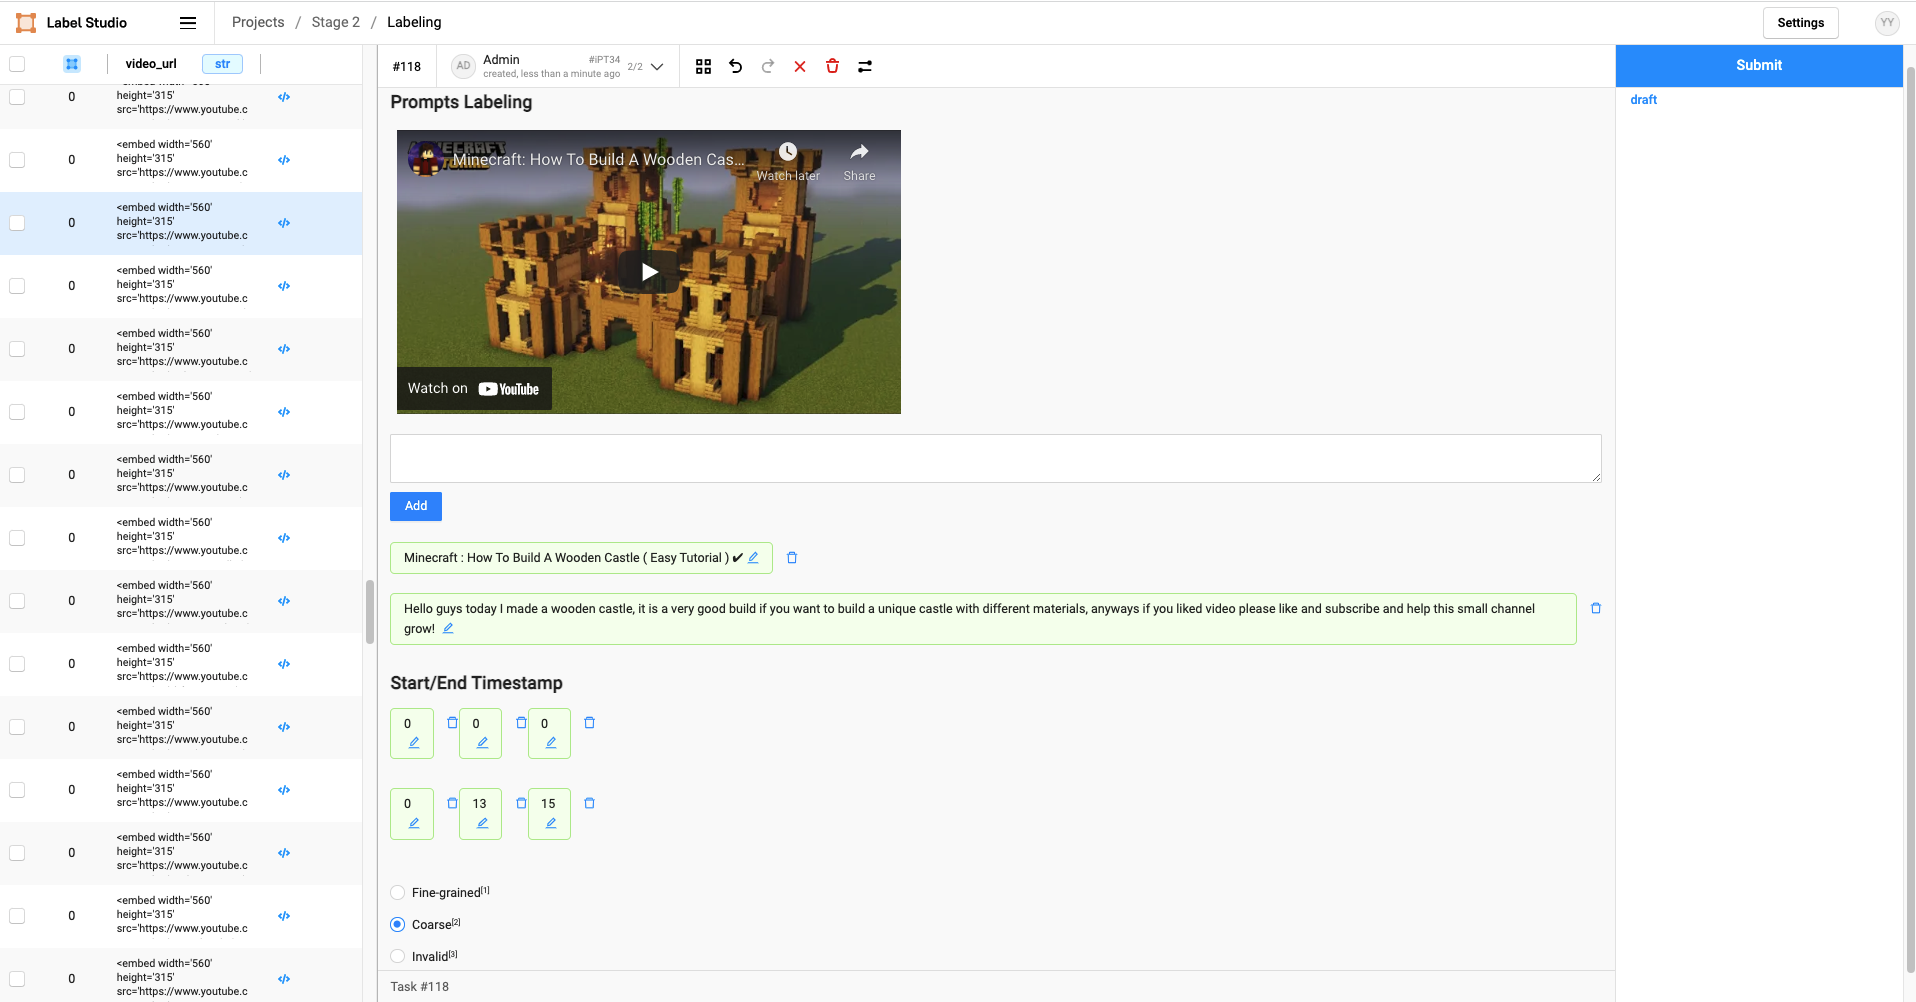
\includegraphics[width=1.0\linewidth]{figs/supp/label_ui-fig.png}
    \vspace{0.02in}
    \caption{Labeling UI to mine tasks from YouTube. A human annotator can choose to reject the video (\textit{Invalid}), adjust the timestamps, select the title, or edit and expand the original description to be the new task goal.}
    \label{supp:fig:label_ui}
\end{figure}
Our YouTube dataset serves the dual purpose of a rich task source, as many human players demonstrate and narrate creative missions in the tutorial playlists. To collect high-quality tasks and accompanying videos, we design a 3-stage pipeline that makes it easy to find and annotate interesting tasks. 
\begin{enumerate}[label=Stage \arabic*:]
    \item We search for YouTube playlists with the key phrases, ``Minecraft Tutorial'' and ``Minecraft Guide''. Then we apply heuristic rules (see Sec.~\ref{supp:sec:dataset-youtube}) to filter out low-quality videos;
    \item We only show the title of the video to a human annotator through a command-line interface, who makes a binary decision to accept or reject it as a potential task. This step is typically very fast, taking a few seconds on average;
    \item For the accepted tasks in stage 2, we design a labeling UI using Label Studio~\cite{labelstudio} that displays the full video and YouTube description. A human annotator can choose to reject the video, adjust the timestamps, select the title, or refine the description to be the task goal (Fig.~\ref{supp:fig:label_ui}). Through this pipeline, we extract 1,042 task ideas from the common wisdom of a huge number of veteran Minecraft gamers. Some examples are ``\textit{make an automated mining machine}'' and ``\textit{grow cactus up to the sky}''.  
\end{enumerate} 


\subsection{GPT-3 Guidance}

We leverage OpenAI's \texttt{GPT-3-davinci} API to automatically generate detailed guidance for a subset of the tasks. Inspired by \cite{kojima2022large}, we adopt the following template to prompt GPT-3: \texttt{How to \{task goal\} in Minecraft? Let's think step by step.} Here are some examples:

The guidance for the task ``\textit{find material and craft a gold pickaxe}'' is \texttt{
1) Find a place with a lot of trees; 
2) Cut down the trees and gather the wood; 
3) Find a place with a lot of stone; 
4) Mine the stone and gather the cobblestone; 
5) Find a place with a lot of iron; 
6) Mine the iron and gather the iron ingots;
7) Find a place with a lot of gold;
8) Mine the gold and gather the gold ingots; 
9) Craft a gold pickaxe.
}

The guidance for the task ``\textit{sail on boat with a sheep}'' is \texttt{
1) Find a boat;
2) Place the sheep in the boat;
3) Right-click on the boat with an empty hand to get in;
4) Use the WASD keys to move the boat. The sheep should stay in the boat.
}

\subsection{Playthrough: Defeat the Ender Dragon}

Our benchmarking suite includes a special task called ``Playthrough''. The agent is initialized bare-handed in a freshly created world and aims to defeat the \textit{Ender dragon}, which is considered the final boss of Minecraft.
This task holds a unique position in our benchmark because killing the dragon means ``beating the game'' in the traditional sense of the phrase, and is considered the most significant achievement for a new player. This boss is optional and plenty of people choose to skip it without affecting their open-ended game experience.

``Playthrough'' is technically a programmatic task, because we can check the simulator state for the defeat of the Ender dragon. However, we decide to create its own category due to the uniqueness as well as the sheer difficulty of the task. The mission requires lots of preparation, exploration, agility, and trial-and-error, which may take a regular human player many days to complete. It would be extremely long horizon (hundreds of thousands of steps) and difficult for an agent to tackle. We consider this one of the moonshot goals in \minedojo.  




\section{Internet-Scale Database}
\label{supp:sec:dataset}

We upload our databases to \texttt{\href{https://zenodo.org}{zenodo.org}}, which is an open repository platform operated by CERN. The data DOIs, URLs, and licenses are listed below. In this section, we describe our database properties and data collection process in details.

\vspace{0.1in}
\resizebox{1.0\textwidth}{!}{%
\begin{tabular}{@{}r|l|l@{}}
\toprule
Database & DOI & License \\ 
\midrule
YouTube & \texttt{\href{https://doi.org/10.5281/zenodo.6641142}{10.5281/zenodo.6641142}} & Creative Commons Attribution 4.0 International (CC BY 4.0) \\
Wiki & \texttt{\href{https://doi.org/10.5281/zenodo.6640448}{10.5281/zenodo.6640448}} & Creative Commons Attribution Non Commercial Share Alike 3.0 Unported \\
Reddit & \texttt{\href{https://doi.org/10.5281/zenodo.6641114}{10.5281/zenodo.6641114}} & Creative Commons Attribution 4.0 International (CC BY 4.0) \\
\bottomrule
\end{tabular}
}
\vspace{0.1in}


\subsection{YouTube Videos and Transcripts}
\label{supp:sec:dataset-youtube}
\begin{figure}
    \centering
    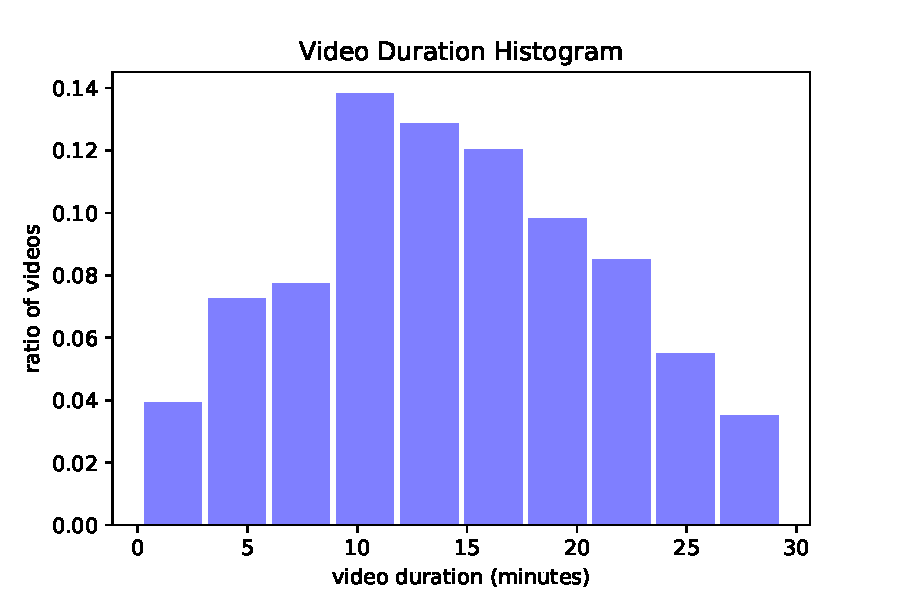
\includegraphics[width=.6\linewidth]{figs/supp/youtube_dist-fig.pdf}
    \caption{Distribution of YouTube video duration. The histogram is trimmed by the 85th percentile to hide much longer videos that can run for many hours.}
    \label{supp:fig:youtube_dist}
\end{figure}

Minecraft is among the most streamed games on YouTube~\cite{gerblick_2021}. Human players have demonstrated a stunning range of creative activities and sophisticated missions that take hours to complete. We collect 33 years worth of video and 2.2B words in the accompanying English transcripts. The distribution of video duration is shown in Fig.~\ref{supp:fig:youtube_dist}.
The time-aligned transcripts enable the agent to ground free-form natural language in video pixels and learn the semantics of diverse activities without laborious human labeling.

We use the official YouTube Data API~\cite{youtubeapi} to collect our database, following the procedure below:
\begin{enumerate}[label=\alph*)]
    \item Search for \textit{channels} that contain Minecraft videos using a list of keywords, e.g., ``Minecraft'', ``Minecraft Guide'', ``Minecraft Walkthrough'', ``Minecraft Beginner''. We do not directly search for videos at this step because there is a limit of total results returned by the API;
    \item Search for all the video IDs uploaded by each channel that we obtain at the previous step. There are many false positives at this step because some channels (like gaming news channel) may cover a range of topics other than Minecraft;
    \item To remove the false positives, we rely on the video category chosen by the user when the video was uploaded and filter out all the videos that do not belong to the Minecraft category;
    \item To curate a language-grounded dataset, we favor videos that have English transcripts, which can be manually uploaded by the user, automatically transcribed from audio, or automatically translated from another language by the YouTube engine. For each video, we filter it out if 1) the view count is less than 100; or 2) the aspect ratio is less 1; or 3) the duration is less than 1 minute long; or 4) marked as age-restricted.
    \item To further clean the dataset and remove potentially harmful contents, we employ the Detoxify~\cite{detoxify} tool to process each video title and description. Detoxify is trained on Wikipedia comments to predict multiple types of toxicity like threats, obscenity, insults, and identity-based hate speech. We delete a video if the toxicity probability in any category is above 0.5.
\end{enumerate}

We release all the video IDs along with metadata such as video titles, view counts, like counts, duration, and FPS. In line with prior practice~\cite{kay2017kinetics}, we do not release the actual MP4 files and transcripts due to legal concerns.

\subsection{Minecraft Wiki}
\label{supp:sec:dataset-wiki}
\begin{figure}
    \centering
    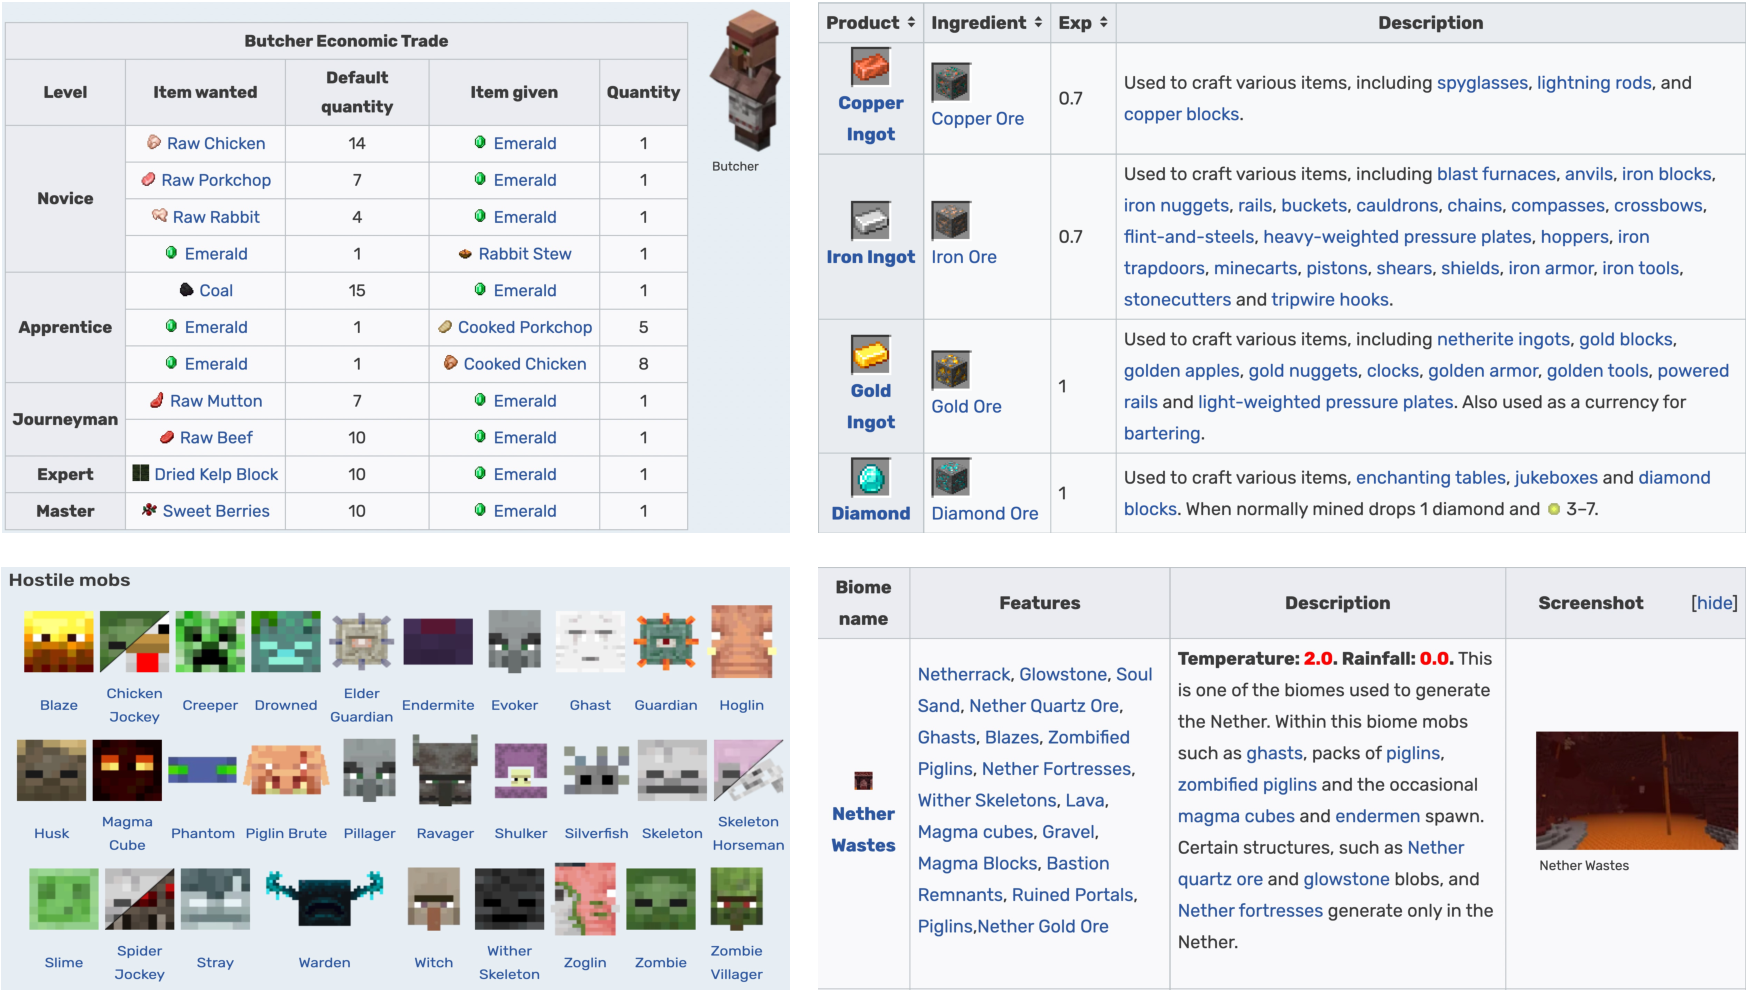
\includegraphics[width=\linewidth]{figs/supp/wiki_supp-fig.pdf}
    \caption{Wiki dataset examples. Closewise order: Villager trade table, mineral ingredient descriptions, monster gallery, and terrain explanation.}
    \label{supp:fig:wiki_supp}
\end{figure}
\begin{figure}
    \centering
    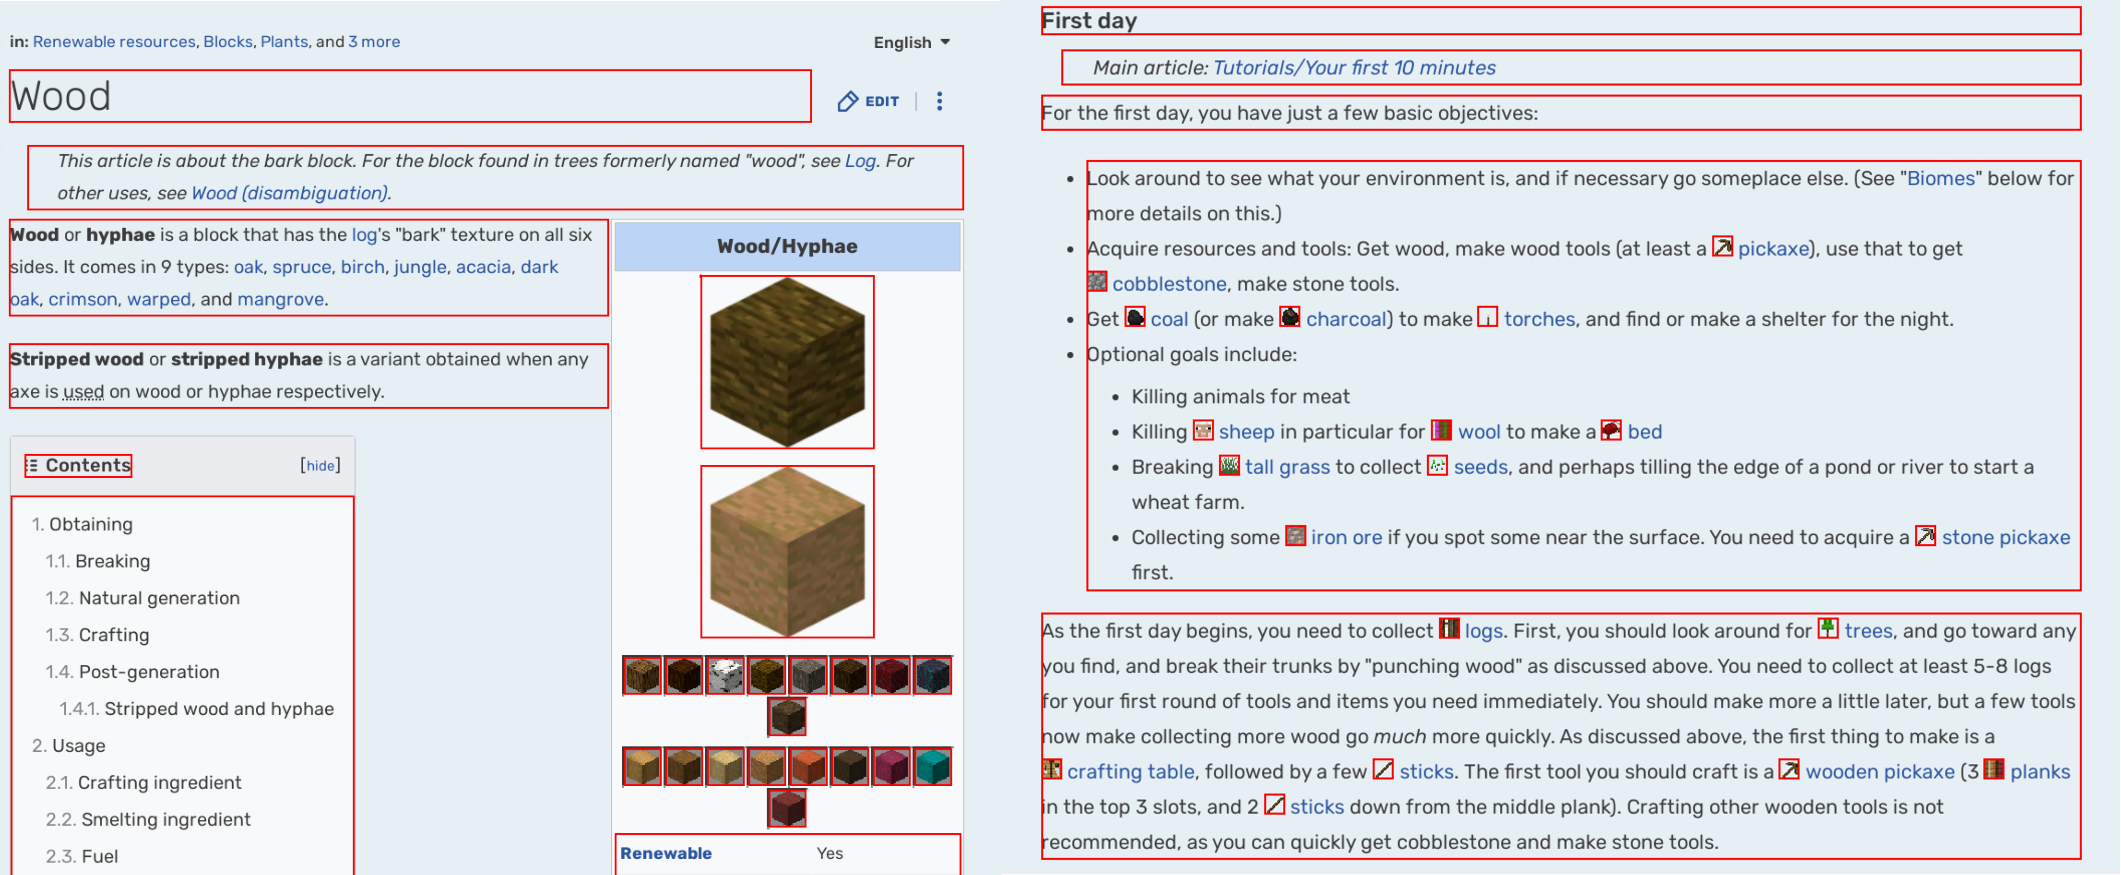
\includegraphics[width=\linewidth]{figs/supp/wiki_bbox-fig.pdf}
    \caption{\Rebuttal{More Wiki database examples with bounding boxes (annotated in red). Left: wood block introduction; right: first day tutorial.}}
    \label{supp:fig:wiki_bbox}
\end{figure}

The Wiki pages cover almost every aspect of the game mechanics, and supply a rich source of unstructured knowledge in multimodal tables, recipes, illustrations, and step-by-step tutorials (example screenshots in Fig.~\ref{supp:fig:wiki_supp} \Rebuttal{and Fig.~\mbox{\ref{supp:fig:wiki_bbox}}}). We use Selenium~\cite{selenium} to scrape 6,735 pages that interleave text, images, tables, and diagrams. 
We elaborate the details of each web element scraped by Selenium:

\begin{enumerate}[label=\alph*)]
    \item \textbf{Screenshot.} Using Selenium's built-in function, we take a full screenshot of the rendered Wiki page in order to preserve the human-readable visual formatting. We also record the bounding boxes of each salient web element on the page. 
    \item \textbf{Text.} We hand-select several HTML tags that likely contain meaningful text data, such as \texttt{p, h1, h2, ul, dl}.
    \item \textbf{Images and Animations.} We download the raw source file of each image element (JPG, PNG, GIF, etc.), as well as the corresponding caption if available. There are also animation effects enabled by JavaScript on the Wiki. We save all image frames in the animation. 
    \item \textbf{Sprites.} Sprite elements are micro-sized image icons that are typically embedded in text to create multimodal tutorials and explanations. We save all the sprites and locate their bounding boxes within the text too. 
    \item \textbf{Tables.} We save the text content and bounding box of each cell that a table element contains. We store the header cells separately as they carry the semantic meaning of each column. A table can be easily reconstructed with the stored text strings and bounding boxes. 
\end{enumerate}


\subsection{Reddit}
\label{supp:sec:dataset-reddit}
\begin{figure}[t]
    \vspace{-0.2in}
    \centering
    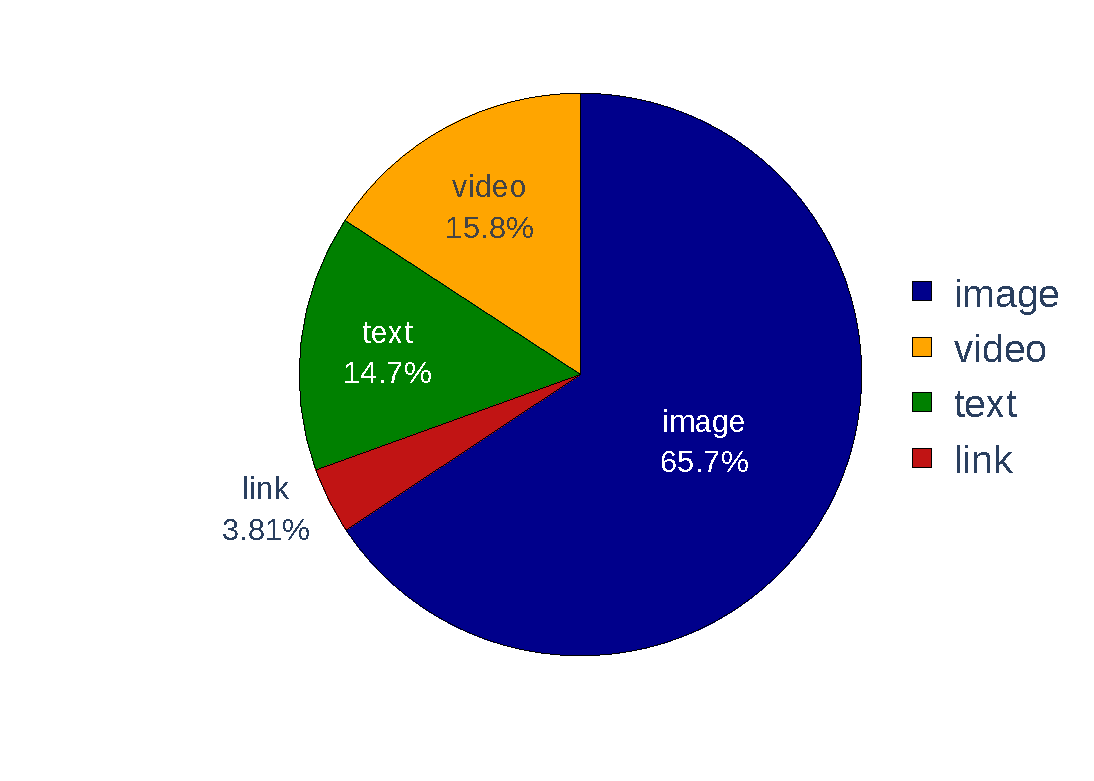
\includegraphics[width=.6\linewidth]{figs/supp/reddit_dist-fig.pdf}
    \vspace{-0.2in}
    \caption{Distribution of Reddit post types.}
    \label{supp:fig:reddit_dist}
\end{figure}
\begin{figure}
    \centering
    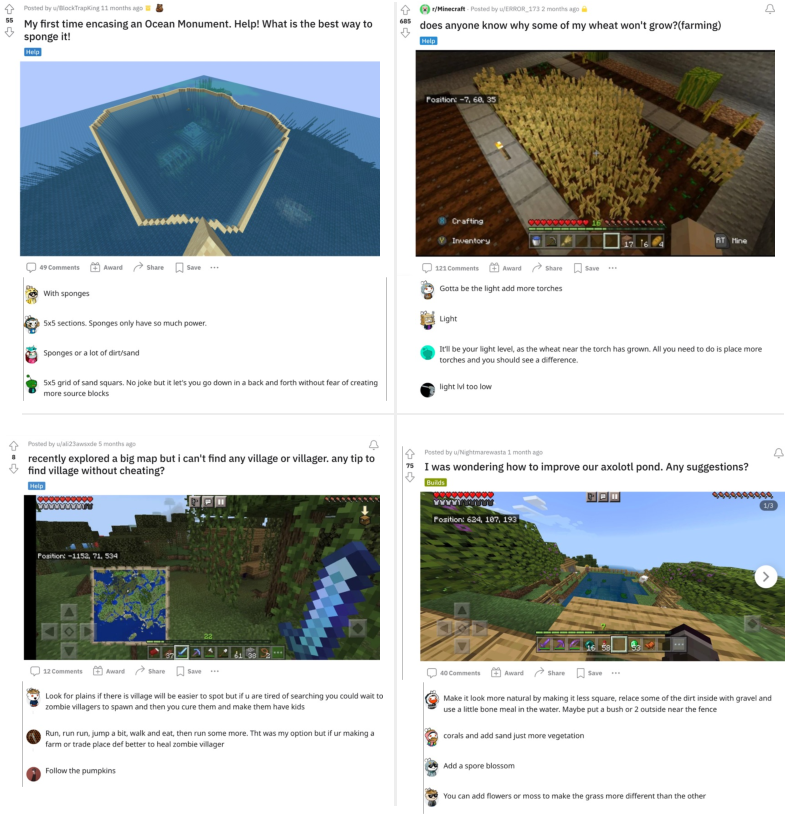
\includegraphics[width=\linewidth]{figs/supp/reddit_supp-fig.pdf}
    \caption{Examples of posts and comment threads from the Reddit database.}
    \label{supp:fig:reddit_supp}
\end{figure}
 There are more than 1M subreddits (i.e., Reddit topics) where people can discuss a wide range of themes and subjects. Prior works use Reddit data for conversational response selection~\cite{al-rfou2016conversational, yang-etal-2018-learning, henderson2019repository} and abstractive summarization~\cite{volske-etal-2017-tl, DBLP:conf/naacl/KimKK19}.
 The \href{https://www.reddit.com/r/minecraft}{r/Minecraft} subreddit contains free-form discussions of game strategies and images/videos showcases of Minecraft builds and creations (examples in Fig.~\ref{supp:fig:reddit_supp}).
The distribution of post types is shown in Fig.~\ref{supp:fig:reddit_dist}. 

To scrape the Reddit contents, we use PRAW~\cite{praw}, a Python wrapper on top of the official Reddit API. Our procedure is as follows:

\begin{enumerate}[label=\alph*)]
    \item Obtain the ID and metadata (e.g. post title, number of comments, content, score) of every post in the ``r/Minecraft'' subreddit since it was created. For quality control, we only consider posts with scores (upvotes) $\geq 5$ and not marked as NSFW.
    \item Determine each post's type. There are 4 native post types - text, image/video, link, and poll. We group text and poll posts together as text posts, and store their body text. 
    For image/video and link posts, we store the source file URLs on external media hosting sites like Imgur and Gfycat. Based on the URL of each link post, we classify it as an image post, a video post or a general link post.
    \item Scrape the comments and store the parent ID of each comment so that we can reconstruct the threaded discussion. 
    \item Similarly to our YouTube database (Sec.~\ref{supp:sec:dataset-youtube}), we run  Detoxify~\cite{detoxify} on the scraped Reddit contents to filter out potentially toxic and harmful posts.
\end{enumerate}

We release all post IDs and their corresponding metadata. We also provide a Python function based on PRAW for researchers to download the post contents after obtaining a license key for the official Reddit API.



\section{\mineclip Algorithm Details}
\label{supp:sec:mineclip}

We implement all our neural networks in PyTorch v1.11 \cite{paszke2019pytorch}. Training \mineclip uses the PyTorch-Lightning framework \cite{falcon2019pytorchlightning}, pre-trained models hosted on HuggingFace \cite{wolf2019huggingfaces}, and the \texttt{x-transformers} library for Transformer variants \cite{wang2021xtransformers}.

\subsection{Video-Text Pair Extraction}

Similar to VideoCLIP~\cite{xu2021videoclip}, we sample 640K pairs of 16-second video snippets and time-aligned English transcripts by the following procedure:

\begin{enumerate}[label=\arabic*)]
    \item Collect a list of keywords corresponding to the supported entities, blocks, and items in Minecraft;
    \item Perform string matching over our YouTube video transcripts to obtain 640K text segments;
    \item For each matched transcript segment, randomly grow it to 16 $\sim$ 77 tokens (limited by CLIP's context length);
    \item Randomly sample a timestamp within the start and end time of the matched transcript as the center for the video clip;
    \item Randomly grow the video clip from the center timestamp to 8 $\sim$ 16 seconds. 
\end{enumerate}


\subsection{Architecture} 
\mineclip architecture is composed of three parts:

\para{Frame-wise image encoder $\phi_I$} We use the ViT-B/16 architecture \cite{dosovitskiy2020image} to compute a 512-D embedding for each RGB frame. We initialize the weights from OpenAI CLIP's public checkpoint \cite{radford2021clip} and only finetune the last two layers during training. The input resolution is  $160 \times 256$, which is different from CLIP's default $224 \times 224$ resolution. We adapt the positional embeddings via bicubic interpolation, which does not introduce any new learnable parameters. 

\para{Temporal aggregator $\phi_a$} Given a sequence of frame-wise RGB features, a temporal aggregator network summarizes the sequence into one video embedding. After the aggregator, we insert two extra layers of residual CLIP Adapter \cite{gao2021clipadapter}. The residual weight is initialized such that it is very close to an identity function at the beginning of training. We consider two variants of $\phi_a$:

\begin{enumerate}
    \item Average pooling (\mineclipavg): a simple, parameter-free operator. It is fast to execute but loses the temporal information, because average pooling is permutation-invariant. 
    \item Self-Attention (\mineclipattn): a 2-layer transformer encoder with 512 embedding size, 8 attention heads, and Gated Linear Unit variant with Swish activation \cite{shazeer2020glu,chowdhery2022palm}. The transformer sequence encoder is relatively slower, but captures more temporal information and achieves better performance in our experiments (Table~\ref{table:core-experiments}).
\end{enumerate}

\begin{table*}
\caption{Training hyperparameters for \mineclip. }
\label{supp:table:hyperparams_mineclip}
\vskip 0.1in
\centering
\resizebox{0.55\textwidth}{!}{%
\begin{tabular}{@{}r|l@{}}
\toprule
Hyperparameter & Value \\ 
\midrule
LR schedule & Cosine with warmup \cite{loshchilov17cosinelr} \\
Warmup steps & 500 \\
Peak LR & 1.5e-4 \\
Final LR & 1e-5 \\
Weight decay & 0.2 \\
Layerwise LR decay & 0.65 \\
Pre-trained layers LR multiplier & $0.5 \times$ \\
Batch size per GPU & 64 \\
Parallel GPUs & 8 \\
Video resolution & $160 \times 256$ \\
Number of frames & 16 \\
Image encoder & \texttt{ViT-B/16} \cite{dosovitskiy2020image} \\

\bottomrule
\end{tabular}
}
\end{table*}



\para{Text encoder $\phi_G$} We use a 12-layer 512-wide GPT model with 8 attention heads \cite{radford2018gpt,radford2019gpt2}. The input string is converted to lower-case byte pair encoding with a 49,152 vocabulary size, and capped at 77 tokens. We exactly follow the text encoder settings in CLIP and initialize the weights from their public checkpoint. Only the last two layers of $\phi_G$ is finetuned during training.  

\subsection{Training}

We train \mineclip on the 640K video-text pairs for 2 epochs. 
We sample 16 RGB frames from each video uniformly, and apply temporally-consistent random resized crop \cite{carreira2017i3d,fan2020rubiks} as data augmentation. 
We use Cosine learning rate annealing with 500 gradient steps of warming up \cite{loshchilov17cosinelr}. We apply a lower learning rate  ($\times 0.5$) on the pre-trained weights and layer-wise learning rate decay for better finetuning \cite{he2021mae}. Training is performed on 1 node of $8 \times$ V100 GPUs with FP16 mixed precision \cite{micikevicius2018mixedprecision} via the PyTorch native \texttt{amp} module. All hyperparameters are listed in Table \ref{supp:table:hyperparams_mineclip}.



\section{Policy Learning Details}
\label{supp:sec:rl}
\begin{algorithm}[t!]
	\caption{PPO-SI Interleaved Training}\label{alg:ppo_si}
	\KwIn{policy $\pi_\theta$, value function $VF(\cdot)$, SI buffer threshold $\Delta$, SI frequency $\omega$}
	Initialize empty SI buffers for all tasks $\mathbf{D}_{SI} \leftarrow \{ \emptyset, \forall T \in \text{training tasks}\}$\;
	Initialize a counter for simulator steps $counter \leftarrow 0$\;
	\While(){not done}{
	    Collect set of trajectories for all tasks $\{\tau_T, \forall T \in \text{training tasks} \}$ by running policy $\pi_\theta$ in (parallel) environments\;
	    \ForAll(){$\mathcal{D}_{SI, T}$}{
	      \uIf{$\tau_T$ is successful}{
	        $\mathcal{D}_{SI, T} \leftarrow \mathcal{D}_{SI, T} \cup \tau_T$
	      }
	      \uElseIf{$\tau_T$'s episode return $\geq \mu_{\text{return}}(\mathcal{D}_{SI, T}) + \Delta \times \sigma_{\text{return}}(\mathcal{D}_{SI, T})$}{
    	      $\mathcal{D}_{SI, T} \leftarrow \mathcal{D}_{SI, T} \cup \tau_T$
	      }
	    }
	    Increase $counter$ accordingly\;
	    Update $\pi_\theta$ following Equation~\ref{eq:ppo_objective}\;
	    Fit $VF(\cdot)$ by regression on mean-squared error\;
	    \uIf{$\mathbbm{1}(counter \bmod \omega = 0)$}{
	        Determine the number of trajectories to sample from each buffer $\#_{\text{sample}} = \min(\{ \vert \mathcal{D}_{SI, T} \vert, \forall T \in \text{training tasks}\})$\;
	        Sample $\#_{\text{sample}}$ trajectories from each buffer in a prioritized manner to construct $\mathcal{D}_{SI}$\;
	        Update $\pi_\theta$ on $\mathcal{D}_{SI}$ with supervised objective\;
	    }
	}
\end{algorithm}

In this section, we elaborate how a trained \mineclip can be adapted as a reward function with two different formulations. We then discuss the algorithm for policy learning. Finally, we demonstrate how we combine self imitation learning and on-policy learning to further improve sample efficiency. 

\subsection{Adapt \mineclip as Reward Function}
\label{supp:sec:rl_mineclip_to_reward}
We investigate two ways to convert \mineclip output to scalar reward, dubbed \direct and \rdelta. The ablation results for \texttt{Animal-Zoo} task group are presented in Table \ref{supp:table:ablation_reward_formulation}.

\para{Direct.} For a task $T$ with the goal description $G$, \mineclip outputs the probability $P_G$ that the observation video semantically corresponds to $G$, against a set of negative goal descriptions $\mathcal{G}^-$. Note that we omit timestep subscript for simplicity. As an example, for the task ``shear sheep'', $G$ is ``shear a sheep'' and $\mathcal{G}^-$ may include negative prompts like ``milk a cow'', ``hunt a sheep'', ``hunt a cow'', etc. 
To compute the \direct reward, we further process the raw probability using the formula  $r = \max( P_G - \frac{1}{N_T}, 0)$ where $N_T$ is the number of prompts passed to \mineclip. $\frac{1}{N_T}$ is the baseline probability of randomly guessing which text string corresponds to the video. We threshold $r$ at zero to avoid highly uncertain probability estimates below the random baseline. We call the variant without the post-processing \direct-Naive: $r = P_G$ as the reward signal for every time step.

\para{Delta.} The \direct formulation yields strong performance when the task is concerned with moving creatures, e.g. farm animals and monsters that run around constantly. However, we discover that \direct is suboptimal if the task deals with static objects, e.g., ``find a nether portal''. Simply using the raw probability from \mineclip as reward can cause the learned agent to stare at the object of interest but fail to move closer and interact. Therefore, we propose to use an alternative formulation, \rdelta, to remedy this issue. Concretely, the reward value at timestep $t$ becomes $r_t = P_{G, t} - P_{G, t - 1}$. We empirically validate that this formulation provides better shaped reward for the task group with static entities. 



\begin{table*}
\caption{Ablation on different \mineclip reward formulations.}
\label{supp:table:ablation_reward_formulation}
\vskip 0.1in
\centering
\begin{tabular}{C{0.1\textwidth}|r|cccccc}

\toprule
Group & Tasks & \direct & \direct-Naive & \rdelta \\ \midrule 

\multirow{4}{*}{\addRoboFig{task1}} & Milk Cow & $\bestscore{64.5 \pm 37.1}$ & $8.6 \pm 1.2$ & $7.6 \pm 5.2$ \\
 & Hunt Cow & $\bestscore{83.5 \pm 7.1\hphantom{0}}$ & $0.0 \pm 0.0$ & $0.0 \pm 0.0$ \\
 & Shear Sheep & $\bestscore{12.1 \pm 9.1\hphantom{0}}$ & $0.8 \pm 0.6$ & $1.8 \pm 1.5$ \\
 & Hunt Sheep & $\bestscore{8.1 \pm 4.1}$ & $0.1 \pm 0.2$ & $0.0 \pm 0.0$ \\
\bottomrule

\end{tabular}
\end{table*}



\subsection{Policy Network Architecture}
Our policy architecture consists of three parts: an input feature encoder, a policy head, and a value function. 
To handle multimodal observations (Sec.~\ref{supp:sec:sim_obs_space}), the feature extractor contains several modality-specific components: 

\begin{itemize}
    \item RGB frame: we use the frozen frame-wise image encoder $\phi_I$ in \mineclip to optimize for compute efficiency and provide the agent with good visual representations from the beginning (Sec.~\ref{sec:method-rl}).
    \item Task goal: $\phi_G$ computes the text embedding of the natural language task goal. 
    \item Yaw and Pitch: compute $\sin(\cdot)$ and $\cos(\cdot)$ features respectively, then pass through an MLP. 
    \item GPS: normalize and featurize via MLP.
    \item Voxel: to process the $3 \times 3 \times 3$ surrounding voxels, we embed discrete block names to dense vectors, flatten them, and pass through an MLP.
    \item Past action: our agent is conditioned on its immediate past action, which is embedded and featurized by MLP. 
\end{itemize}

Features from all modalities are concatenated, passed through another fusion MLP, and finally fed into the policy head and value function head. 
We use an MLP to model the policy head that maps from the input feature vectors to the action probability distribution. We use another MLP to estimate the value function, conditioned on the same input features. 

\subsection{RL Training}
\label{sec:appendix_rl_training}

\para{PPO.} We use the popular PPO algorithm ~\cite{schulman2017proximal} (Proximal Policy Optimization) as our RL training backbone. PPO is an on-policy method that optimizes for a surrogate objective while ensuring that the deviation from the previous policy is relatively small. PPO updates the policy network by
\begin{equation}
    \underset{\theta}{\text{maximize}}\;\mathbb{E}_{s,a\sim\pi_{\theta_{\text{old}}}} L(s, a, \theta_\text{old}, \theta),
\end{equation} where
\begin{equation}
    L(s, a, \theta_\text{old}, \theta) = \min \left(\frac{\pi_{\theta}(a|s)}{\pi_{\theta_\text{old}}(a|s)} A^{\pi_{\theta_\text{old}}}(s, a), \text{clip}\left(\frac{\pi_{\theta}(a|s)}{\pi_{\theta_\text{old}}(a|s)}, 1-\epsilon, 1+\epsilon\right)A^{\pi_{\theta_\text{old}}}(s, a)\right).
    \label{eq:ppo_objective}
\end{equation}
$A$ is an estimator of the advantage function (GAE~\cite{DBLP:journals/corr/SchulmanMLJA15} in our case) and $\epsilon$ is a hyperparameter that controls the deviation between the new policy and the old one.

\para{Self Imitation Learning.} We apply self-imitation learning \cite{oh2018self} (SI) to further improve sample efficiency because computing the reward with \mineclip in the loop makes the training more expensive. Self-imitation learning is essentially supervised learning on a buffer $\mathcal{D}_{SI}$ of good trajectories generated by the agent's past self. In our case, the trajectories are generated by the behavior policy during PPO rollouts, and only added to $\mathcal{D}_{SI}$ if it is a \emph{successful} trial or if the episodic return exceeds a certain threshold. Self imitation optimizes $\pi_\theta$ for the objective  
$\mathcal{J}_{SI} = \mathbb{E}_{s, a \sim \mathcal{D}_{SI}} \log \pi_\theta (a \vert s)$ 
with respect to $\theta$.

We alternate between the PPO phase and the SI phase. 
A pseudocode of our interleaved training procedure is given in Algorithm~\ref{alg:ppo_si}. We use a \emph{prioritized} strategy to sample trajectories from the buffer $\mathcal{D}_{SI}$. Specifically, we assign equal probability to all successful trajectories. Unsuccessful trajectories can still be sampled but with lower probabilities proportional to their episodic returns. 

In Fig. \ref{supp:fig:ablation_si}, we demonstrate that adding self-imitation dramatically improves the stability, performance, and sample efficiency of RL training in \minedojo.  

\begin{figure*}[t!]
     \centering
     \begin{subfigure}[b]{0.49\linewidth}
         \centering
         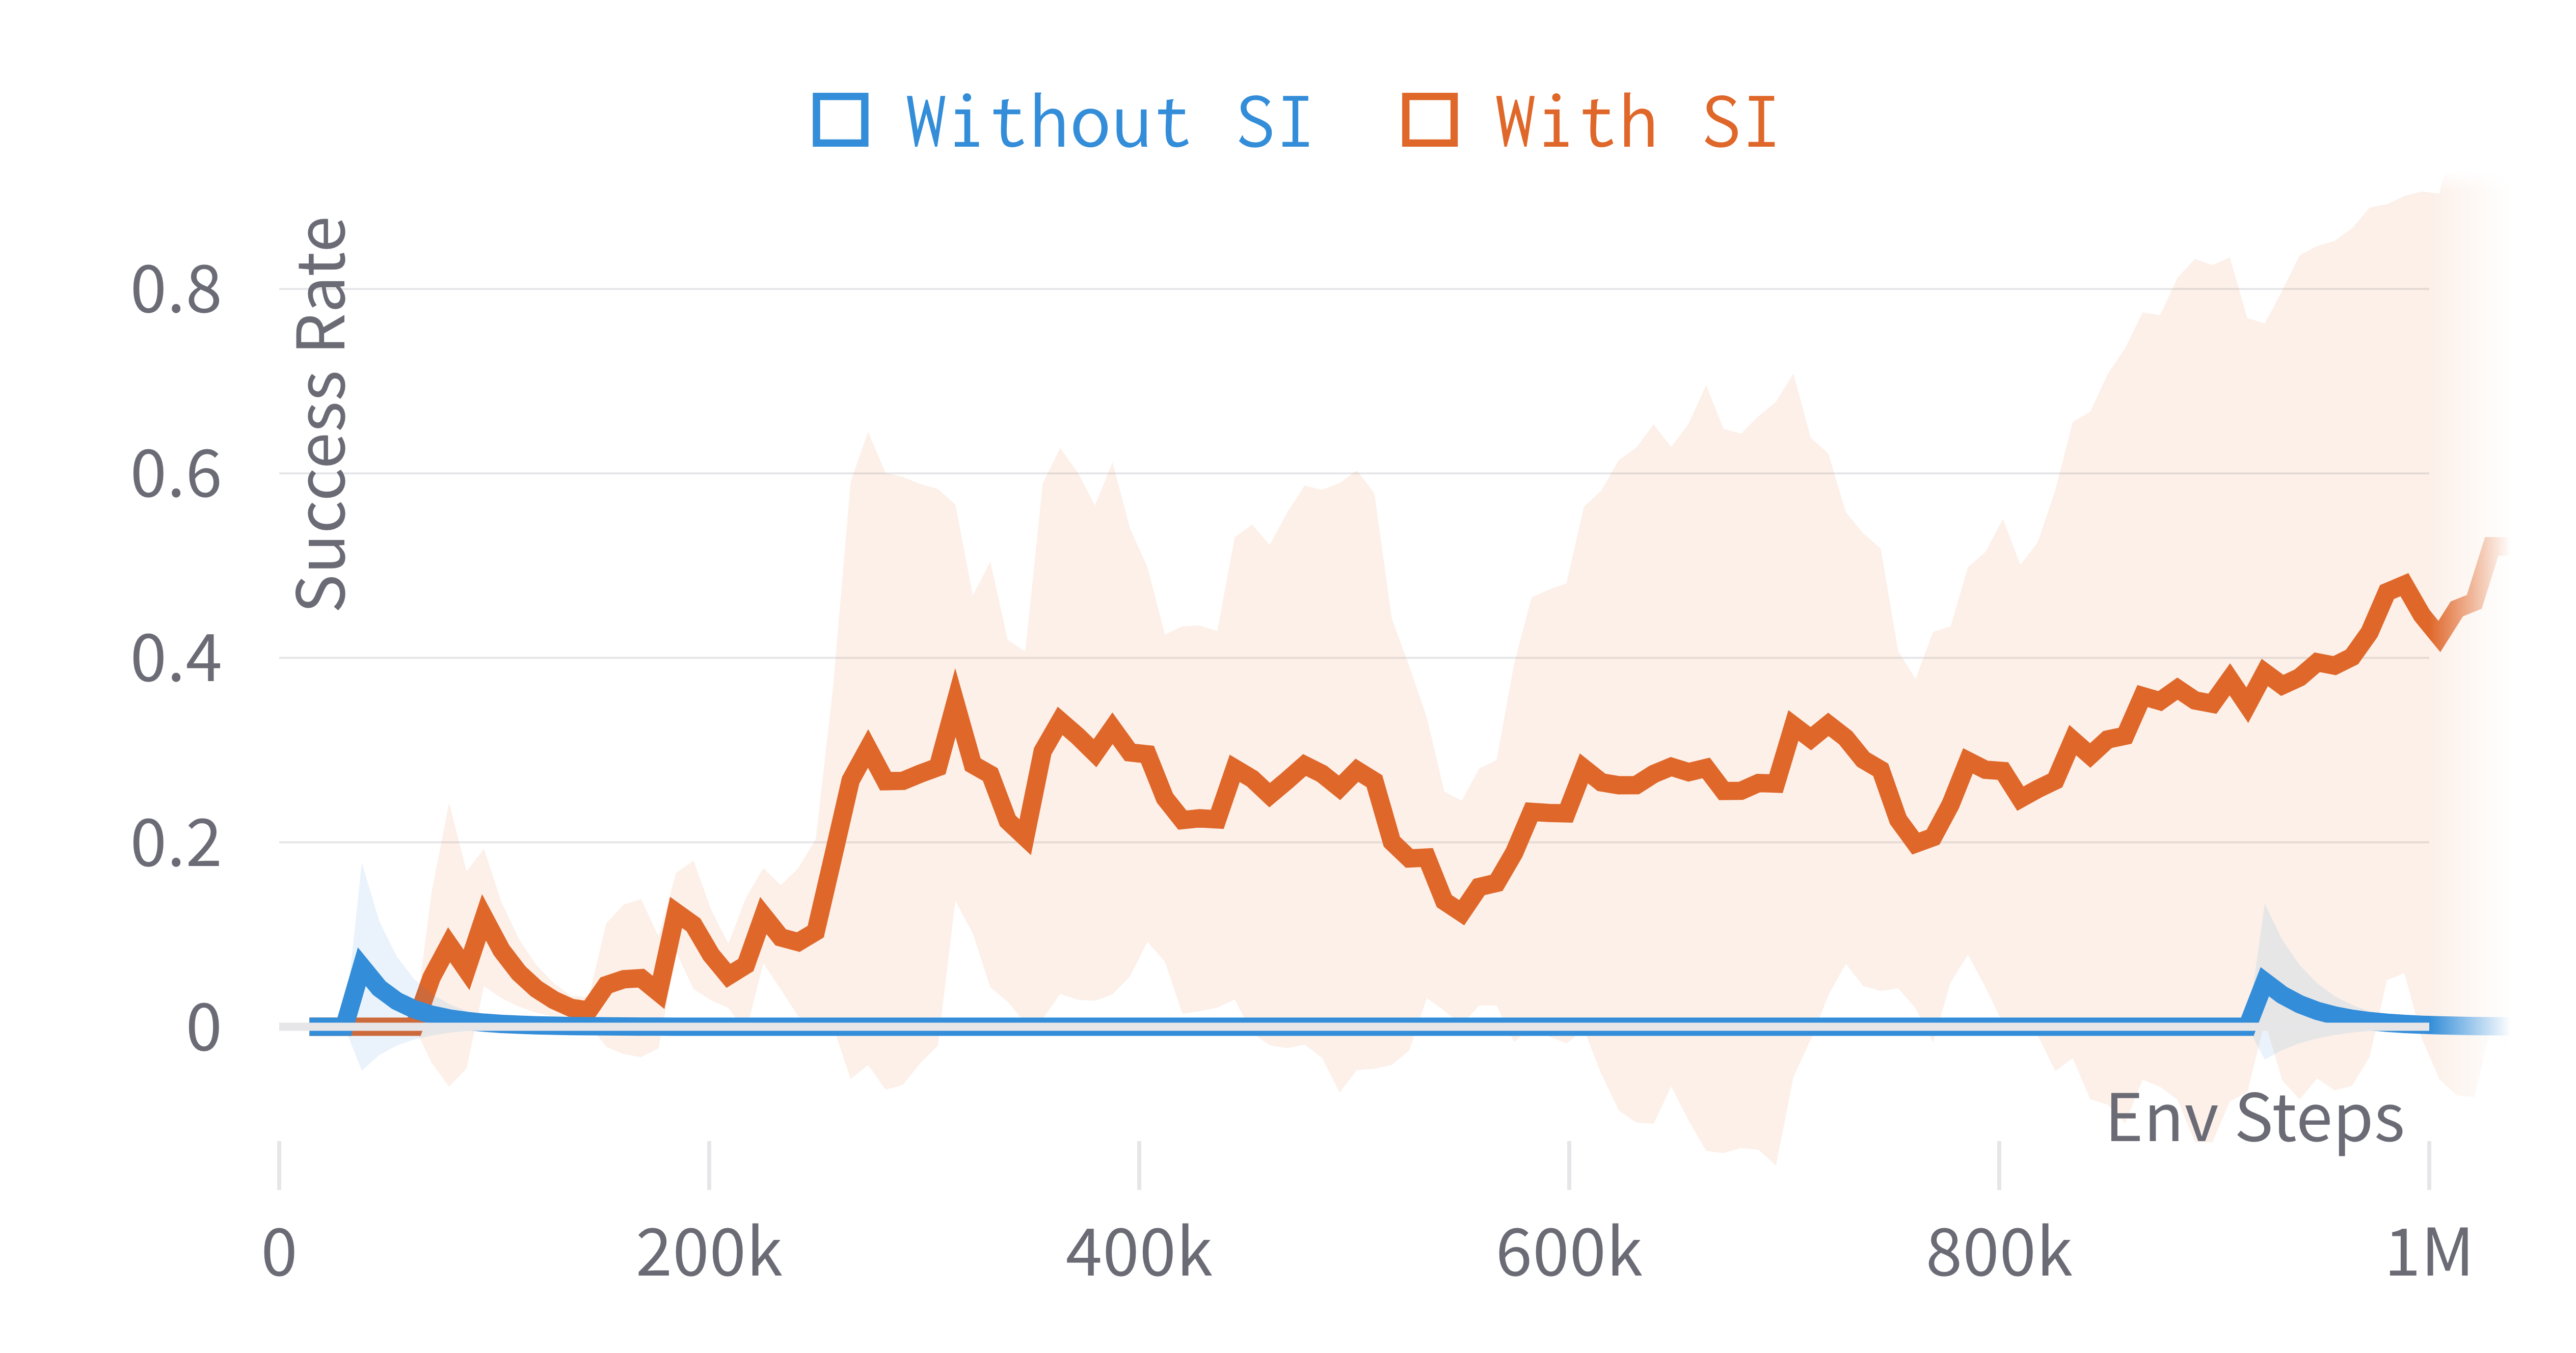
\includegraphics[width=\textwidth]{figs/supp/si_ablation_milk_cow.png}
         \caption{``Milk Cow''}
         \label{fig:si_ablation_milk_cow}
     \end{subfigure}
     \hfill
     \begin{subfigure}[b]{0.49\linewidth}
         \centering
         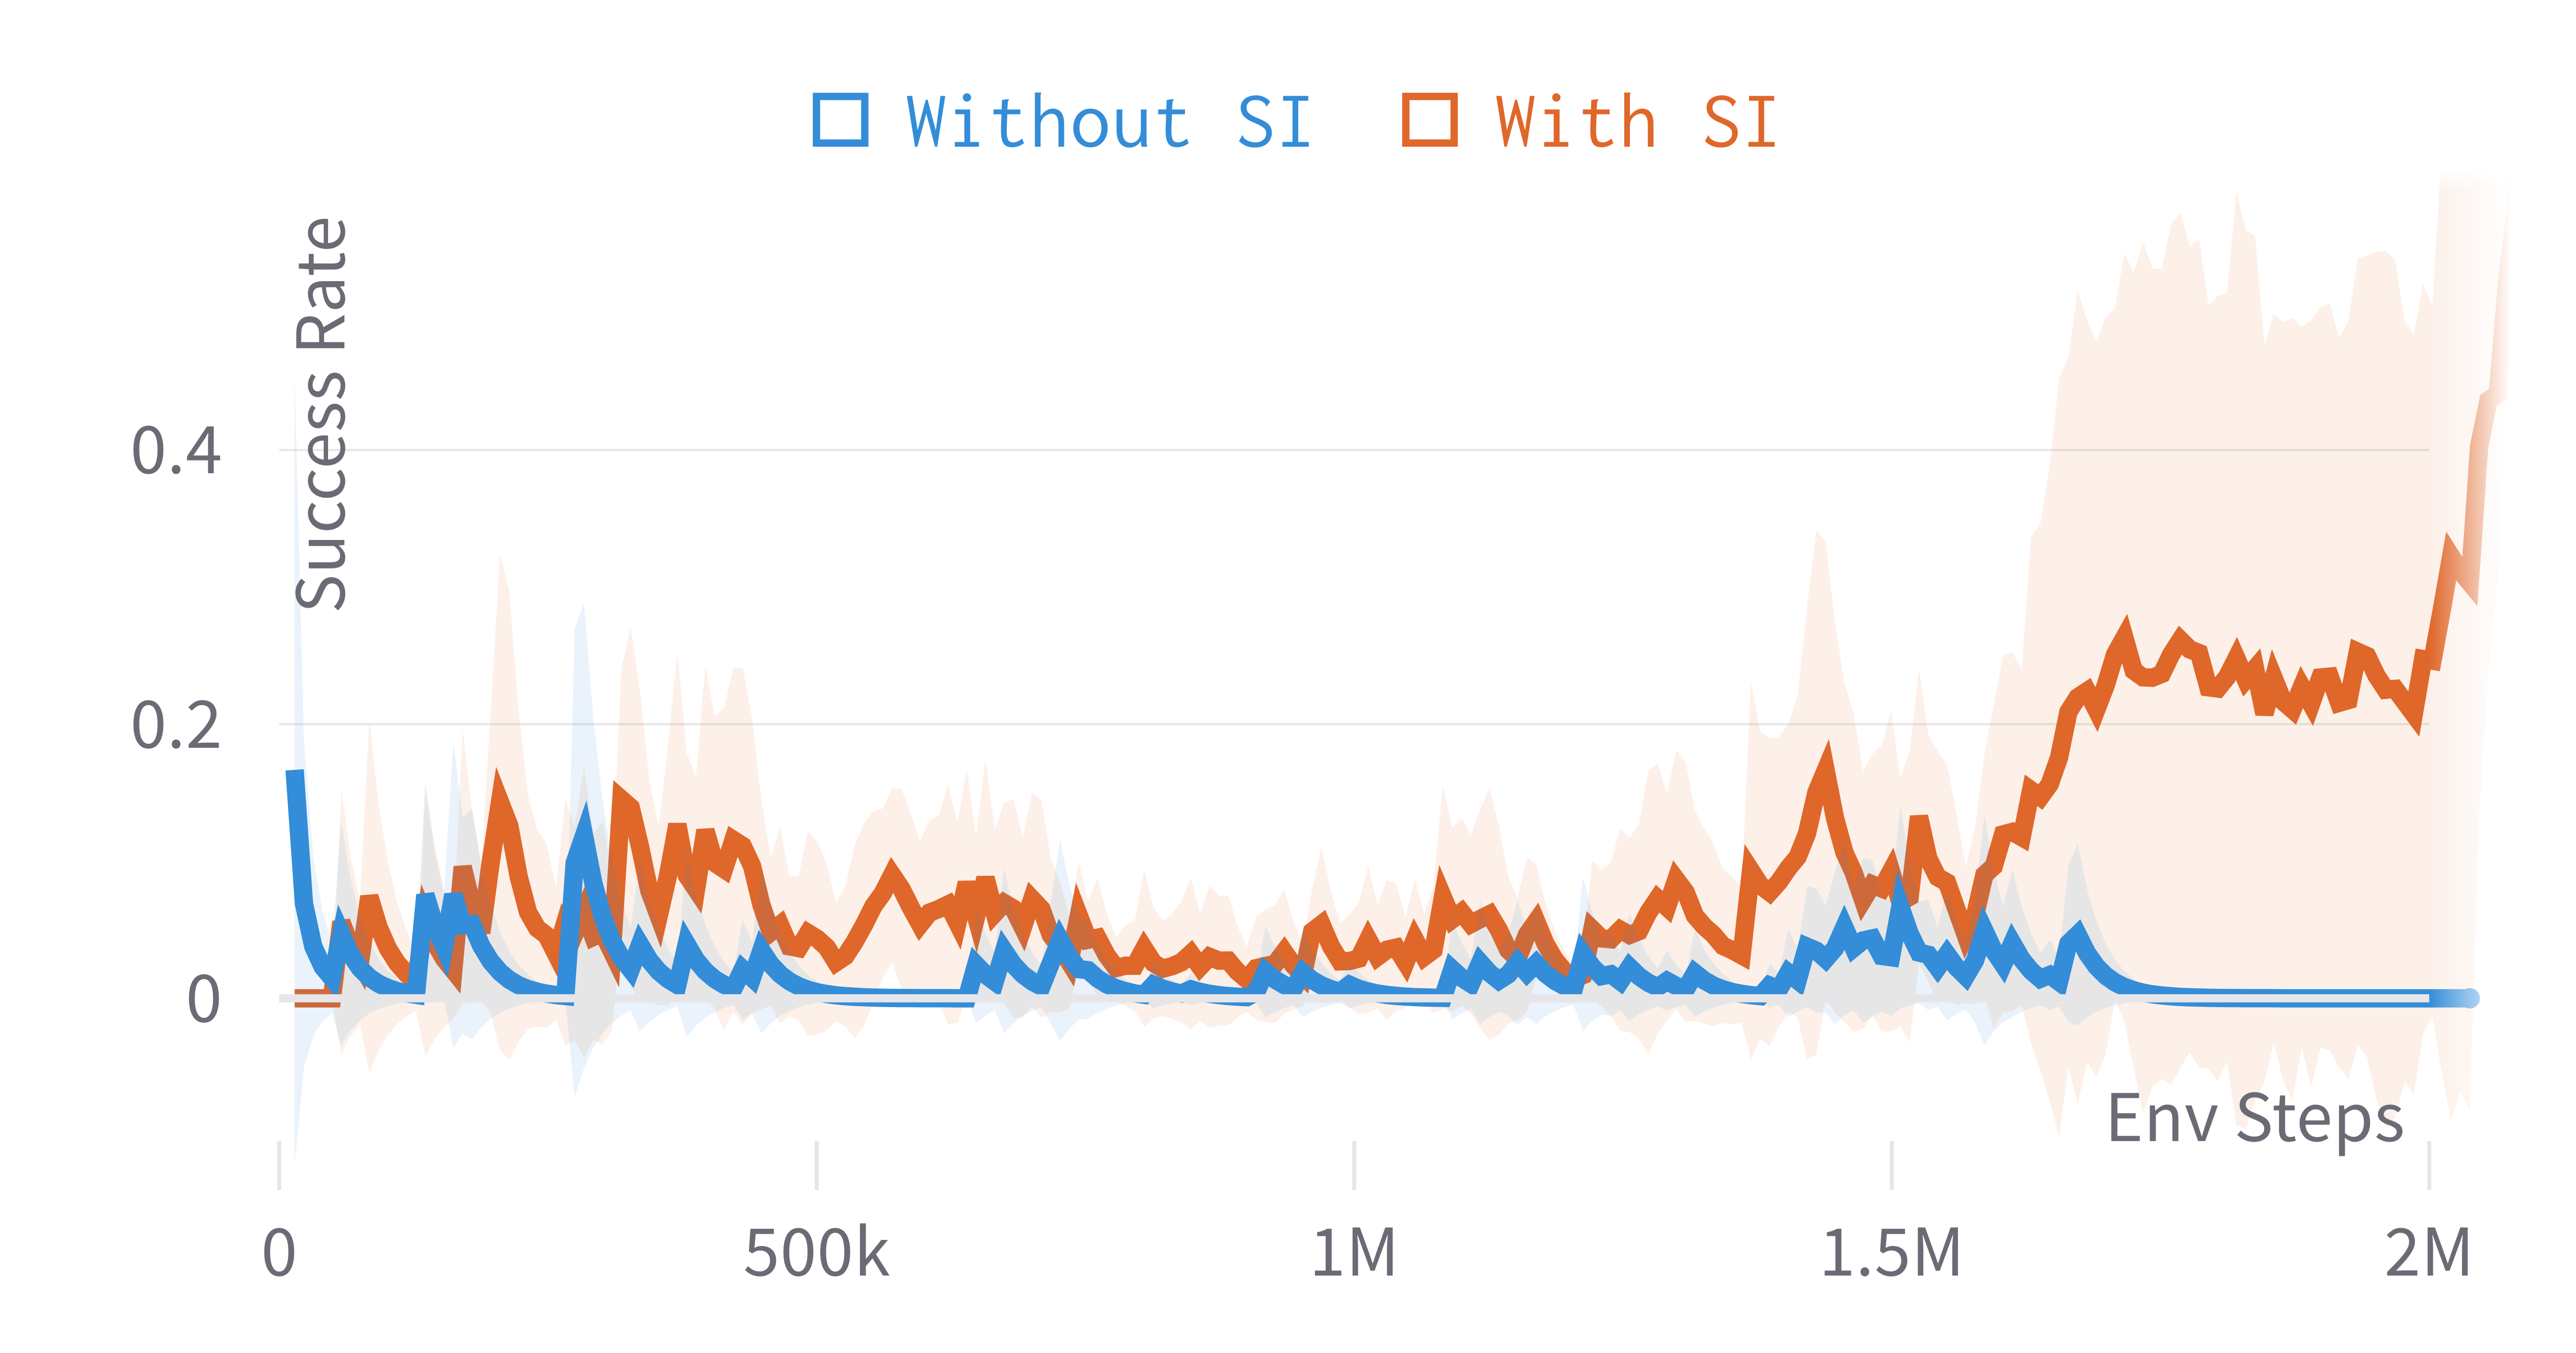
\includegraphics[width=\textwidth]{figs/supp/si_ablation_shear_sheep.png}
         \caption{``Shear Sheep''}
         \label{fig:si_ablation_shear_sheep}
     \end{subfigure}
    \caption{Adding the self imitation technique \cite{oh2018self} significantly improves the performance of RL training in \minedojo.}
    \label{supp:fig:ablation_si}
\end{figure*}



\section{Experiment Details}
\label{supp:sec:experiments}

\subsection{Task Details}
\label{supp:sec:task_details}
We experiment with three task groups with four tasks per group. We train one multi-task agent for each group. In this section, we describe each task goals, initial setup, and the manual dense-shaping reward function.

\para{\underline{Animal Zoo}:} 4 Programmatic tasks on hunting or harvesting resource from animals. We spawn various animal types (pig, sheep, and cow) in the same environment to serve as distractors. It is considered a failure if the agent does not take action on the correct animal specified by the prompt.

\begin{itemize}
    \item  \textbf{Milk Cow}: find and approach a cow, then obtain milk from it with an empty bucket. The prompt is \texttt{milk a cow}. We initialize the agent with an empty bucket to collect milk. We also spawn sheep, cow, and pig nearby the agent. The manual dense reward shaping is a navigation reward based on geodesic distance obtained from privileged LIDAR. The combined reward passed to PPO can be formulated as $r_t = \lambda_{\text{nav}}\max(d_{\text{min}, t - 1} - d_{\text{min}, t}, 0) + \lambda_{\text{success}} \mathbbm{1}(\text{milk collected})$, where $\lambda_{\text{nav}} = 10$ and $\lambda_{\text{success}} = 200$. $d_{\text{min}, t} = \min(d_{\text{min}}, d_{t})$ where $d_{\text{min}}$ denotes the minimal distance to the cow that the agent has achieved so far in the episode history. 
    \item \textbf{Hunt Cow}: find and approach a cow, then hunt with a sword. The cow will run away so the agent needs to chase after it. The prompt is \texttt{hunt a cow}. We initialize the agent with a diamond sword. The manual dense reward shaping consists of two parts, a valid attack reward and a navigation reward based on geodesic distance obtained from privileged LIDAR. Mathematically, the reward is $r_t = \lambda_{\text{attack}}\mathbbm{1}(\text{valid attack}) + \lambda_{\text{nav}}\max(d_{\text{min}, t - 1} - d_{\text{min}, t}, 0) + \lambda_{\text{success}} \mathbbm{1}(\text{cow hunted})$, where $\lambda_{\text{attack}} = 5$, $\lambda_{\text{nav}} = 1$, and $\lambda_{\text{success}} = 200$. We additionally reset $d_\text{min}$ every time the agent hits the cow to encourage the chasing behavior. 
    \item \textbf{Shear Sheep}: find and approach a sheep, then collect wool from the sheep with a shear. The prompt is \texttt{shear a sheep}. We initialize the agent with a shear. The manual dense reward shaping is a navigation reward based on geodesic distance obtained from the privileged LIDAR sensor, similar to ``Milk Cow''.
    \item \textbf{Hunt Sheep}: find and approach a sheep, then hunt with a sword. The sheep will run away so the agent needs to chase after it. An episode will terminate once any entity is hunted. The prompt is \texttt{hunt a sheep}. We initialize the agent with a diamond sword. The manual dense reward shaping consists of two parts, a valid attack reward and a navigation reward based on geodesic distance obtained from the privileged LIDAR sensor, similar to ``Hunt Cow''.
\end{itemize}

\para{\underline{Mob Combat}:} fight 4 different types of hostile monsters: Spider, Zombie, Zombie Pigman (a creature in the \textit{Nether} world), and Enderman (a creature in the \textit{End} world). The prompt template is \texttt{"Combat \{monster\}"}.
For all tasks within this group, we initialize the agent with a diamond sword, a shield, and a full suite of diamond armors. The agent is spawned in the \textit{Nether} for Zombie Pigman task, and in the \textit{End} for Enderman.
The manual dense-shaping reward can be expressed as $r_t = \lambda_{\text{attack}} \mathbbm{1}(\text{valid attack}) + \lambda_{\text{success}} \mathbbm{1}(\texttt{\{monster\}}\text{ hunted})$ where $\lambda_{\text{attack}} = 5$ and $\lambda_{\text{success}} = 200$.

\para{\underline{Creative}:} 4 tasks that do not have manual dense reward shaping or code-defined success criterion.

\begin{itemize}
    \item \textbf{Find Nether Portal}: find and move close to a Nether Portal, then enter the \textit{Nether} world through the portal. The prompt is \texttt{find a nether portal}. 
    \item \textbf{Find Ocean}: find and move close to an ocean. The prompt is \texttt{find an ocean}. 
    \item \textbf{Dig Hole}: dig holes in the ground. The prompt is \texttt{dig a hole}. We initialize the agent with an iron shovel.
    \item \textbf{Lay Carpet}: lay down carpets to cover the wooden floor inside a house. The prompt is \texttt{put carpets on the floor}. We initialize the agent with a number of carpets in its inventory. 
\end{itemize}

\Rebuttal{Note that we categorize ``Find Nether Portal'' and ``Find Ocean'' as Creative tasks even though they seem similar to object navigation \mbox{\cite{batra2020objectnav}}. While finding terrains and other structures is semantically well defined, it is not easy to define a function to evaluate success automatically because the simulator does not have the exact location information of these structures given a randomly generated world. In principle, we can make a sweep by querying each chunk of voxels in the world to recognize the terrains, but that would be prohibitively expensive. Therefore, we opt to use MineCLIP as the reward signal and treat these tasks as Creative.} 

\begin{table*}[t!]
\caption{Hyperparameters in RL experiments. ``\texttt{\{state\}} MLP'' refers to MLPs to process observations of compass, GPS, and voxel blocks. ``Embed Dim'' denotes the same dimension size used to embed all discrete observations into dense vectors.}
\label{supp:table:hyperparams_rl}

\centering
\resizebox{\textwidth}{!}{%
\begin{tabular}{rrll|rccc}
\toprule
\multicolumn{4}{c|}{\multirow{2}{*}{NN Architecture}}       & \multicolumn{4}{c}{Training}                                                                                                         \\ \cline{5-8} 
\multicolumn{4}{c|}{}                                       & Hyperparameter              & \multicolumn{1}{c|}{\texttt{Animal-Zoo}}         & \multicolumn{1}{c|}{\texttt{Mob-Combat}}         & \texttt{Creative}           \\ \hline
RGB Feature Size                & \multicolumn{3}{c|}{512}  & Learning Rate               & \multicolumn{1}{c|}{$10^{-4}$}          & \multicolumn{1}{c|}{$10^{-4}$}          & $10^{-4}$          \\
Task Prompt Feature Size        & \multicolumn{3}{c|}{512}  & Cosine Decay Minimal LR     & \multicolumn{1}{c|}{$5 \times 10^{-6}$} & \multicolumn{1}{c|}{$5 \times 10^{-6}$} & $5 \times 10^{-6}$ \\
\texttt{\{state\}} MLP Hidden Size           & \multicolumn{3}{c|}{128}  & $\gamma$                    & \multicolumn{1}{c|}{$0.99$}             & \multicolumn{1}{c|}{$0.99$}             & $0.99$             \\
\texttt{\{state\}} MLP Output Size           & \multicolumn{3}{c|}{128}  & Entropy Weight (Stage 1)    & \multicolumn{1}{c|}{$5 \times 10^{-3}$} & \multicolumn{1}{c|}{$5 \times 10^{-3}$} & $5 \times 10^{-3}$ \\
\texttt{\{state\}} MLP Hidden Depth          & \multicolumn{3}{c|}{2}    & Entropy Weight (Stage 2)    & \multicolumn{1}{c|}{$10^{-2}$}          & \multicolumn{1}{c|}{N/A}                & $10^{-2}$          \\
Embed Dim                       & \multicolumn{3}{c|}{8}    & PPO Optimizer               & \multicolumn{1}{c|}{Adam}               & \multicolumn{1}{c|}{Adam}               & Adam               \\
Num Feature Fusion Layers       & \multicolumn{3}{c|}{1}    & SI Learning Rate            & \multicolumn{1}{c|}{$10^{-4}$}          & \multicolumn{1}{c|}{$10^{-4}$}          & $10^{-4}$          \\
Feature Fusion Output Size      & \multicolumn{3}{c|}{512}  & SI Cosine Decay Minimal LR  & \multicolumn{1}{c|}{$10^{-6}$}          & \multicolumn{1}{c|}{$10^{-6}$}          & $10^{-6}$          \\
Prev Action Conditioning        & \multicolumn{3}{c|}{True} & SI Epoch                    & \multicolumn{1}{c|}{10}                 & \multicolumn{1}{c|}{10}                 & 10                 \\
Policy Head Hidden Size         & \multicolumn{3}{c|}{256}  & SI Frequency (Env Steps)    & \multicolumn{1}{c|}{100K}               & \multicolumn{1}{c|}{100K}               & 100K               \\
Policy Head Hidden Depth        & \multicolumn{3}{c|}{3}    & SI Optimizer                & \multicolumn{1}{c|}{Adam}               & \multicolumn{1}{c|}{Adam}               & Adam               \\
VF Hidden Size        & \multicolumn{3}{c|}{256}  & SI Buffer Threshold         & \multicolumn{1}{c|}{$2 \sigma$}         & \multicolumn{1}{c|}{$2 \sigma$}         & $0.5 \sigma$       \\
VF Hidden Depth        & \multicolumn{3}{c|}{3}    & PPO Buffer Size             & \multicolumn{1}{c|}{100K}               & \multicolumn{1}{c|}{100K}               & 100K               \\
                                & \multicolumn{3}{c|}{}     & Frame Stack                 & \multicolumn{1}{c|}{1}                  & \multicolumn{1}{c|}{1}                  & 1                  \\
                                & \multicolumn{3}{c|}{}     & VF Loss Weight              & \multicolumn{1}{c|}{0.5}                & \multicolumn{1}{c|}{0.5}                & 0.5                \\
                                & \multicolumn{3}{c|}{}     & GAE $\lambda$               & \multicolumn{1}{c|}{0.95}               & \multicolumn{1}{c|}{0.95}               & 0.95               \\
                                & \multicolumn{3}{c|}{}     & Gradient Clip               & \multicolumn{1}{c|}{10}                 & \multicolumn{1}{c|}{10}                 & 10                 \\
                                & \multicolumn{3}{c|}{}     & PPO $\epsilon$              & \multicolumn{1}{c|}{0.2}                & \multicolumn{1}{c|}{0.2}                & 0.2                \\
                                & \multicolumn{3}{c|}{}     & Action Smooth Weight        & \multicolumn{1}{c|}{$10^{-7}$}          & \multicolumn{1}{c|}{$10^{-7}$}          & $10^{-7}$          \\
                                & \multicolumn{3}{c|}{}     & Action Smooth Window Size   & \multicolumn{1}{c|}{3}                  & \multicolumn{1}{c|}{3}                  & 3                  \\
                                & \multicolumn{3}{c|}{}     & \mineclip Reward Formulation & \multicolumn{1}{c|}{\direct}     & \multicolumn{1}{c|}{\direct}     & \rdelta              \\ \bottomrule
\end{tabular}


}
\end{table*}


\subsection{Observation and Action Space}

We use a subset of the full observation and action space listed in Sec.~\ref{supp:sec:sim_obs_space} and \ref{supp:sec:sim_action_space}, because the tasks in our current experiments do not involve actions like crafting or inventory management. Our observation space consists of RGB frame, compass, GPS, and Voxels.

Our action space is a trimmed version of the full action space. It consists of movement control, camera control, ``use'' action, and ``attack'' action, which add up to 89 discrete choices. Concretely, it includes 81 actions for discrete camera control ($9 \times 9$ resulted from the Cartesian product between yaw and pitch, each ranges from $-60$ degree to $60$ degree with a discrete interval of $15$ degree). It also includes 6 movement actions (forward, forward + jump, jump, back, move left, and move right) and 2 functional actions of ``use'' and ``attack''. Note that the ``no-op'' action is merged into the 81 camera actions. 


\subsection{RL Training}
All hyperparameters used in our RL experiment are listed in Table~\ref{supp:table:hyperparams_rl}. We visualize the learned behaviors of 4 tasks in Figure~\ref{fig:behavior_visualization}. Demos of more tasks can be found on our website \weburl.

\para{Action smoothing.} 
Due to the stochastic nature of PPO, we observe a lot of action jittering in the agent's behavior during training. This leads to two negative effects that degrade the learning performance: 1) exploration difficulty due to inconsistent action sequence. For example, the agent may be required to take multiple consecutive \texttt{attack} actions in order to complete certain tasks; and 2) rapidly switching different movement and camera motions result in videos that are highly non-smooth and disorienting. This causes a domain gap from the training data of \mineclip, which are typically smooth human gameplay videos. Therefore, the reward signal quality deteriorates significantly.

To remedy the issue, we impose an action smoothing loss to be jointly optimized with the PPO objective (Eq.~\ref{eq:ppo_objective}) during training. Concretely, consider a sliding window $\mathcal{W}$ with window size $\vert \mathcal{W} \vert$ that contains $\vert \mathcal{W} \vert$ consecutive action distributions $\mathcal{W} = \{\pi_{t - \vert \mathcal{W} \vert + 1}, \pi_{t - \vert \mathcal{W} \vert + 2}, \ldots, \pi_{t} \}$, the action smoothing loss is defined as 
\begin{equation}
    \mathcal{L}_{\text{smooth}} = \frac{1}{\vert \mathcal{W} \vert} \sum_{i = 1}^{\vert \mathcal{W} \vert - 1} KL(\pi_t \Vert \pi_{t - \vert \mathcal{W} \vert + i}),
\end{equation}
where $KL(\cdot)$ denotes Kullback–Leibler divergence. 
 
\para{Multi-stage training for multi-task RL.} 
Due to hardware limitations, we are not able to run a large number of parallel simulators for all tasks in a task group. Therefore, we adopt a multi-stage strategy to split the tasks and train them sequentially with a single policy network. For the task groups \texttt{Animal-Zoo} and \texttt{Creative}, we split the four tasks into two stages of two parallel training tasks each. We carry over the self-imitation buffers when switching to the next stage. We also follow the recommended practice in \cite{nikishin2022primacy} and reset the policy head at the beginning of stage 2 to encourage exploration and reduce overfitting. We adopt a similar replay buffer balancing strategy as \cite{gupta2022metamorph} to prevent any task from dominating the training. 

\subsection{Evaluation}
\label{supp:sec:mineclip_complex_creative}
In this section, we elaborate on our human and automatic evaluation procedure for Creative tasks.
We first ask the human annotators to manually label 100 successful and 100 failure trajectories. This produces a combined dataset of 200 trajectories with groundtruth binary labels to evaluate the learned reward functions.  
On this dataset, we run \mineclip to produce step-wise rewards and compute a score that averages over each trajectory. We then apply K-means clustering with $K = 2$ to all scores and determine a decision boundary $\delta$ from the mean of the two centroids. A trajectory with a score greater than $\delta$ is classified as successful, and vice versa for failure. In this way, we essentially convert \mineclip to a binary classifier. 
The quality of \mineclip can be measured by the F1 score of its binary classification output against the human labels. We demonstrate that \mineclip has high agreements with humans (Table \ref{table:eval-metric-quality}), and thus qualifies as an effective automatic evaluation metric for Creative tasks in the absence of human judges. 

To further investigate \mineclip{}'s evaluation on more complex Creative tasks,
we annotate 50 YouTube video segments each for 5 more tasks that are much more semantically complex: ``build a farm'', `` build a fence'', ``build a house'', ``ride a minecart'', and ``build a swimming pool''. We then run \mineclip evaluation on these videos against a negative set. As shown in Table \ref{table:supp-mineclip-eval-more}, though not perfect, \mineclip generally has a positive agreement with human judgment. We note that the current \mineclip is a proof-of-concept step in leveraging internet data for automated evaluation, and further scaling on more training data and parameters may lead to more improvements. Meanwhile, human judgment remains a useful and important alternative \cite{openai2022dalle2,saharia2022imagen}.

\begin{table}[t!]
\caption{
\Rebuttal{\mbox{\mineclip{}'s} evaluation on more complex Creative tasks. 
Numbers represent F1 scores between \mbox{\mineclip}'s evaluation on tasks success and human labels. Scaled to percentage for better readability.}
}
\label{table:supp-mineclip-eval-more}
\vskip 0.1in
\centering

\resizebox{1\textwidth}{!}{
\begin{tabular}{r|ccccccc}
\toprule
 Tasks & Build a Farm & Build a Fence & Build a House & Ride a Minecart & Build a Swimming Pool  \\ \midrule 

 Ours (Attn) & $\bestscore{78.7}$ & $\bestscore{91.4}$ & $\bestscore{63.7}$ & $95.9$ & $85.0$\\

 Ours (Avg) & $73.4$ & $83.1$ & $37.4$ & $\bestscore{96.9}$ & $\bestscore{94.7}$\\
 
 \openaiclip & $62.5$ & $24.5$ & $52.9$ & $70.0$ & $71.7$\\

\bottomrule
\end{tabular}
}
\end{table}



\section{Limitations and Potential Societal Impact}

Unlike human demonstrations \cite{vinyals2019alphastar} or offline RL datasets \cite{fu2020d4rl}, our YouTube dataset contains only the video screen observations but not the actual control actions. This allows us to scale up the dataset tremendously, but at the same time poses a challenge to imitation learning algorithms that require observation-action pairs to learn. 
Our proposed algorithm, \mineclip, side-steps this problem by learning a reward model, but we believe that directly inferring the human expert policy from YouTube is another important direction complementary to our approach. There are promising techniques that can potentially overcome this limitation, such as the Learning-from-Observation (LfO) family of algorithms \cite{torabi2019lfosurvey,torabi2018behavioral,stadie2017thirdperson,edwards2018imitatinglatent}. 

Our database is scraped from the internet, which inevitably contains offensive YouTube videos or toxic Reddit posts. While we have made our best effort to filter out these harmful contents (Sec.~\ref{supp:sec:dataset-youtube}), there can still be undesirable biases and toxicity that elude our automatic filters. Furthermore, we advocate the use of large pre-trained language models in our main paper, and \mineclip is finetuned from the pre-trained weights of OpenAI CLIP \cite{radford2021clip}. These foundation models are known to contain harmful stereotypes and generate hateful commentary \cite{brown2020gpt3,bommasani2021foundation,gehman2020realtoxicityprompts}. We ask the researchers who will use our code and database to exercise their best judgment during new model development to avoid any negative social impact.   
